\section{Klasse diagrammer}

På klasse diagrammet FlightPathHandling ses de tre overordnet klasser hvilket udgør pakken FlightPathHandling pakken som vist på figur \ref{fig:pakke_diagram}.

\vspace{-5pt}
%kommentar
\begin{figure}[H]
	\centering
	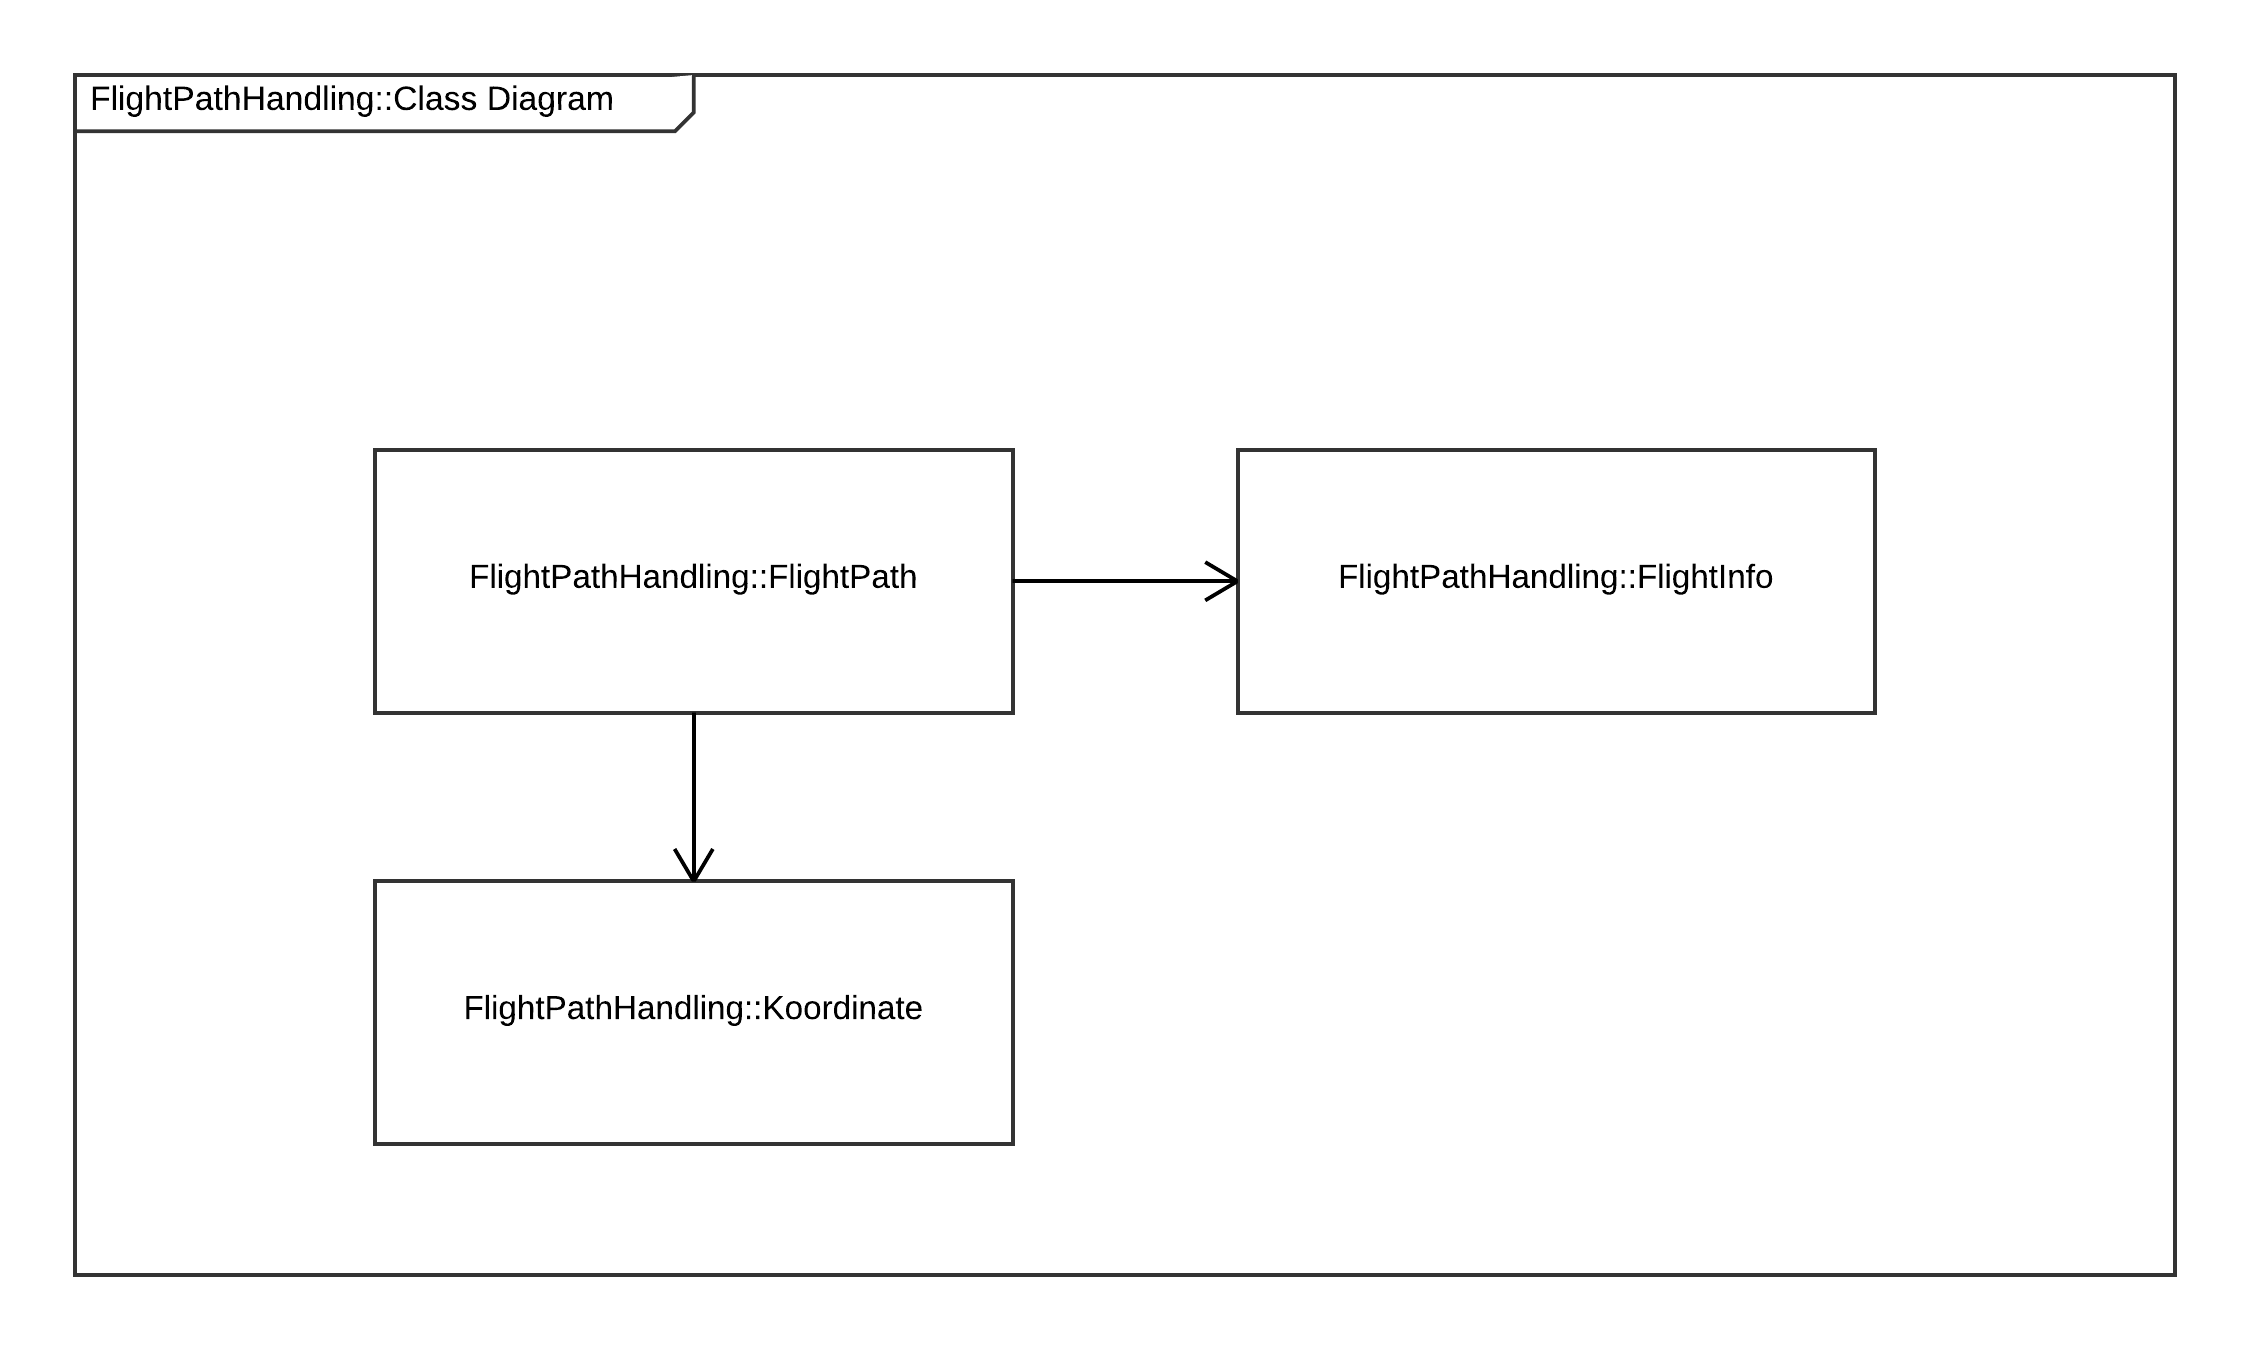
\includegraphics[width=0.7\textwidth]{Billeder/klasse_diagrammer/FlightPathHandlingDiagram.png}
	\vspace{-5pt}
	\caption{FlightPathHandling klasse diagram}
	\label{fig:FlightPathHandling_klasse_diagram}
\end{figure}

\textbf{FlightPath}\\
Klassen FlightPath bruger både FlightInfo og Coordinate klasserne til at udgøre en FlightPath.

\textbf{Coordinate}\\
Coordinate klassen håndtere det GPS koordinater som brugeren ønsker dronen skal flyve til.

\textbf{FlightInfo}\\
FlightInfo klassen håndtere data om ruten så som flyvehøjde, dato for flyvning mm. 

\newpage
Klasse diagrammet viser hvilket klasser som udgør UserHandling pakken som vist på figur \ref{fig:pakke_diagram}.

\vspace{-5pt}
%kommentar
\begin{figure}[H]
	\centering
	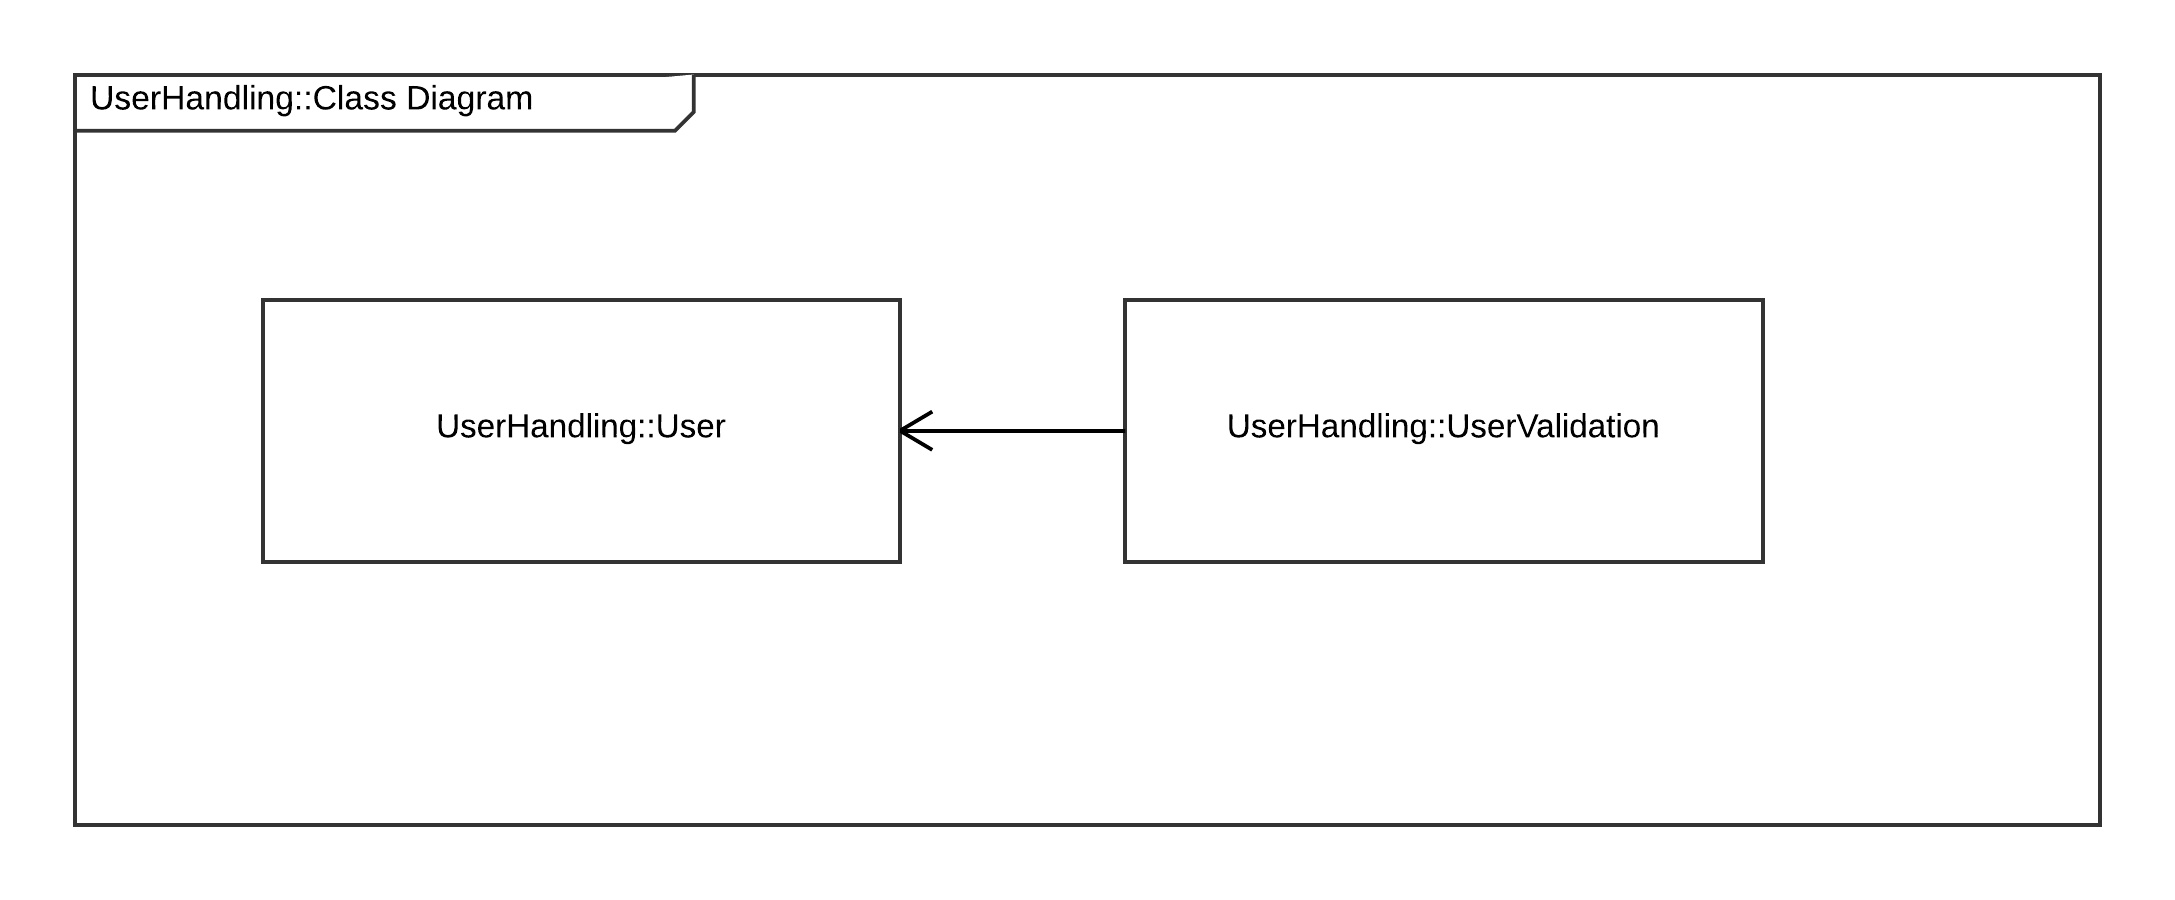
\includegraphics[width=0.7\textwidth]{Billeder/klasse_diagrammer/UserHandlingDiagram.png}
	\vspace{-5pt}
	\caption{UserHandling klasse diagram}
	\label{fig:UserHandling_klasse_diagram}
\end{figure}

\textbf{User}\\
User klassen indeholder alle data om brugerne i systemet. Klassen bliver også brugt af UserValidation i forbindelse med login/log out.

\textbf{UserValidation}\\
UserValidation klassen har ansvaret for at validere en user når der bliver forsøgt login.\\


Klasse diagrammet viser hvilket klasser som udgør DatabaseHandling pakken som vist på figur \ref{fig:pakke_diagram}.

\vspace{-5pt}
%kommentar
\begin{figure}[H]
	\centering
	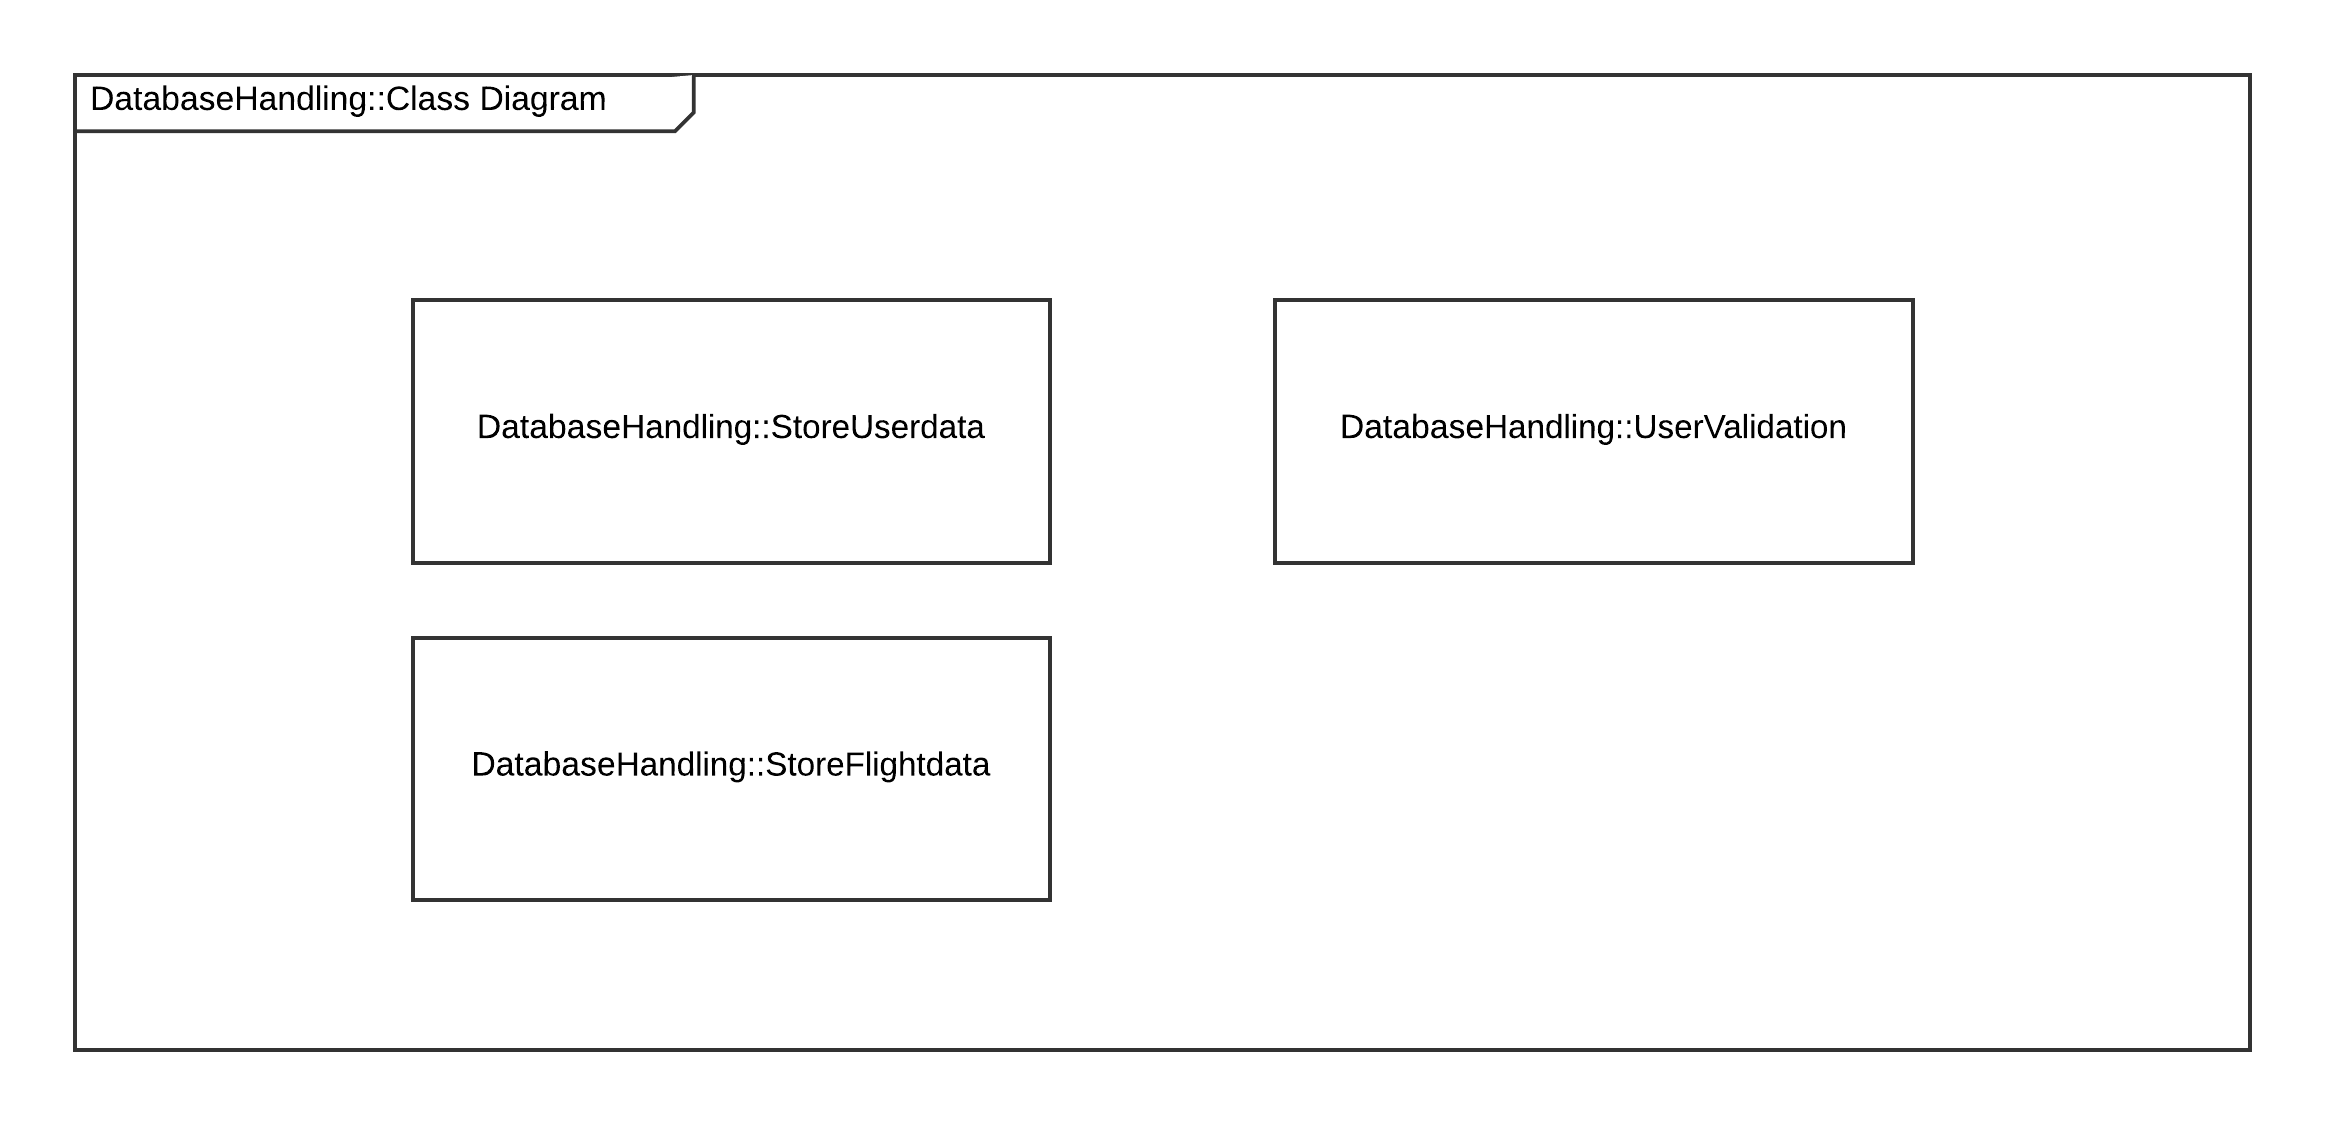
\includegraphics[width=0.7\textwidth]{Billeder/klasse_diagrammer/DatabaseHandling.png}
	\vspace{-5pt}
	\caption{DatabaseHandling klasse diagram}
	\label{fig:DatabaseHandling_klasse_diagram}
\end{figure}

\vspace{-5pt}
%kommentar
\begin{figure}[H]
	\centering
	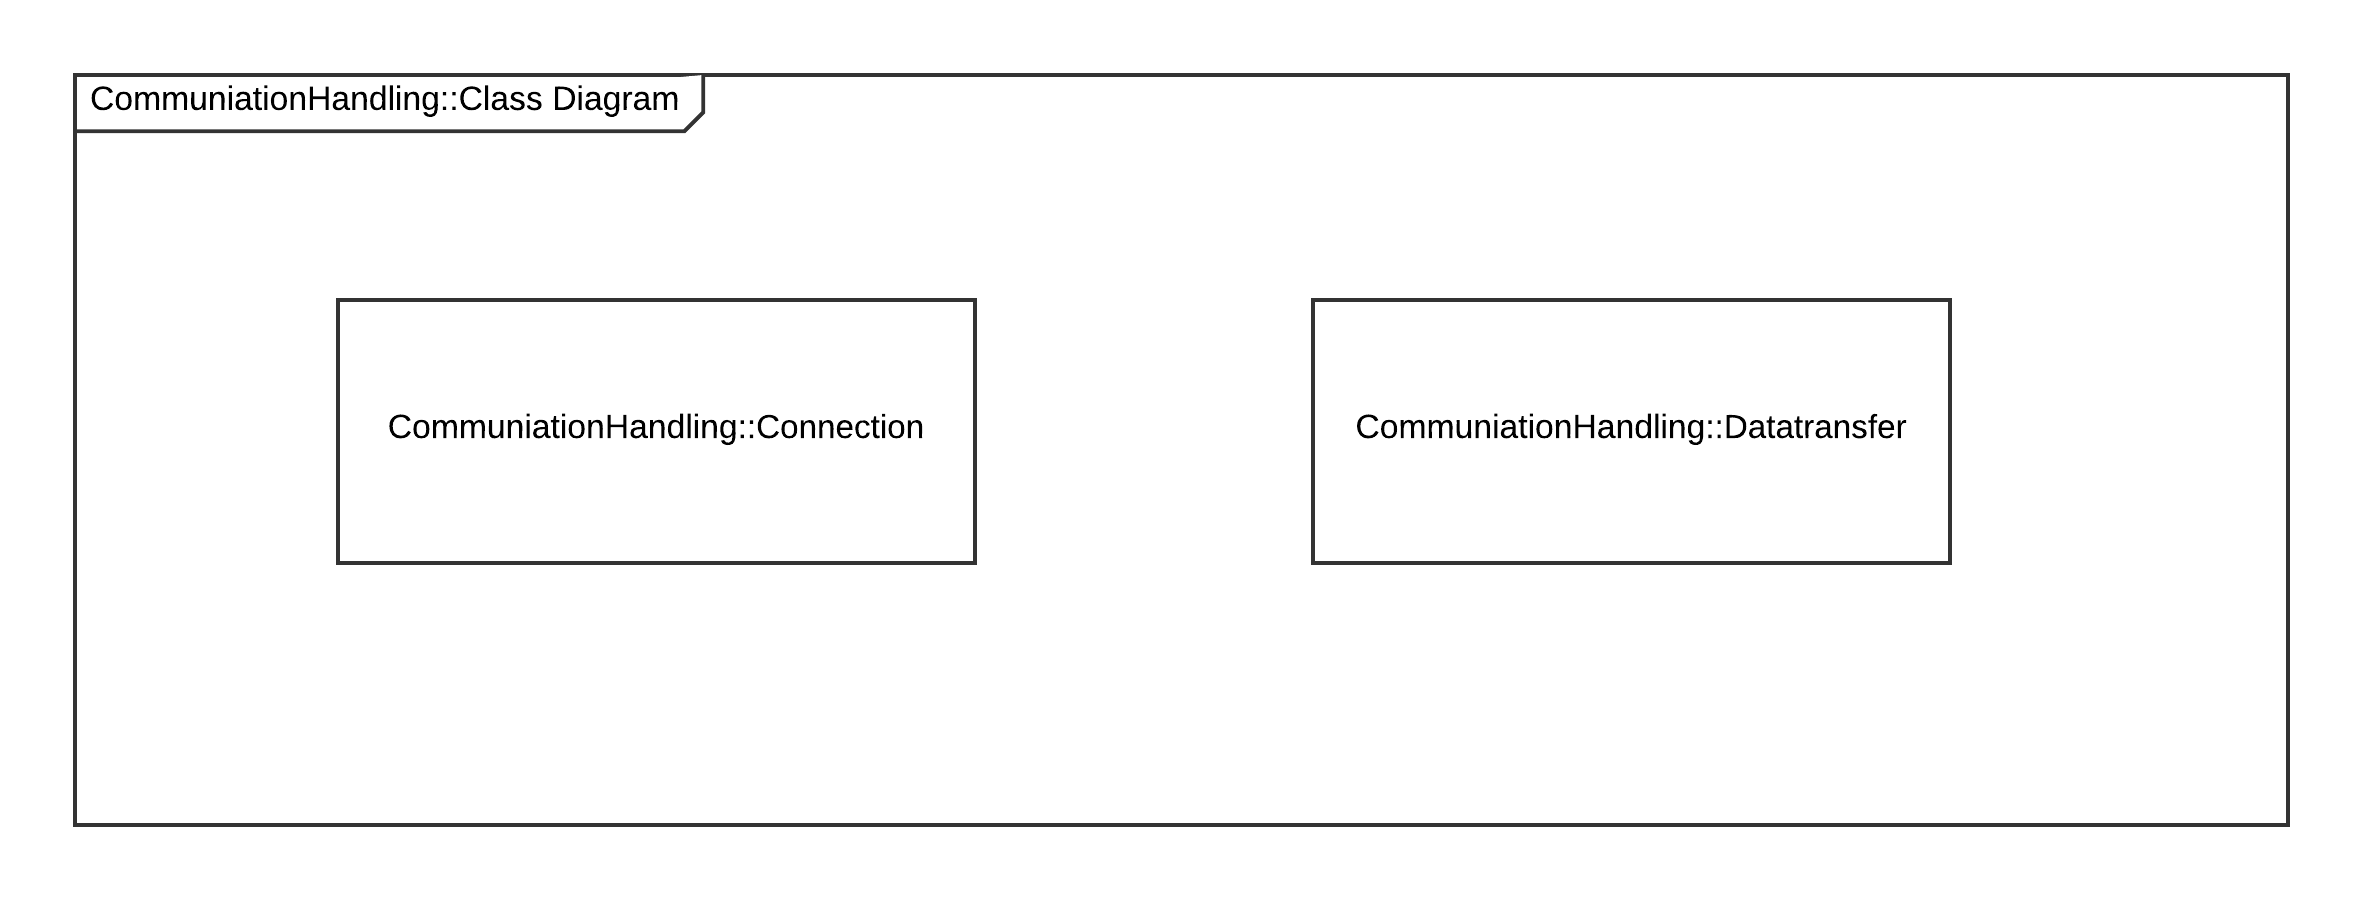
\includegraphics[width=0.7\textwidth]{Billeder/klasse_diagrammer/CommunicationHandling.png}
	\vspace{-5pt}
	\caption{CommunicationHandling klasse diagram}
	\label{fig:CommunicationHandling_klasse_diagram}
\end{figure}